

% \documentclass[article,tikz,border=3mm]{standalone}
\documentclass{article}
\usepackage{blindtext}

% setting up the margin of the paper 
\usepackage[a4paper, total={6.5in, 9in}]{geometry}

% setup for font family for the title/section name, for text font you have set ti seperately
\usepackage[T1]{fontenc}
\usepackage{lmodern}

% package for tables, this package I don't why always stay at the top of the document
\usepackage{tikz}
% I don't know what is this for right now
\usepackage{mathtools,eqparbox}

% not sure for right now 
\usepackage{array}
\usepackage{blkarray, bigstrut} % matrix label

% index package 
\usepackage{imakeidx}
\makeindex % this line is mandatory

% package for basic symbol characters $/rhd$
% https://artofproblemsolving.com/wiki/index.php/LaTeX:Symbols
\usepackage{latexsym}

\usepackage{amsmath}
\usepackage[makeroom]{cancel} % cancel out single item by using \cancel{}

\usepackage{pgfplots} % 2 dimensional ploting
\usepackage{pgfplotstable}
\pgfplotsset{compat = newest}
\usetikzlibrary{datavisualization.formats.functions} % 2 dimensional ploting
\usetikzlibrary{tikzmark} % arrow for pointing
\usepackage{tikz-3dplot} % 3 dimensional plot
\newcommand{\Arrow}[1]{%
\parbox{#1}{\tikz{\draw[->](0,0)--(#1,0);}}
} % for \Arrow in tikz package

\hbadness=10000  % silence the warning for \\ breaking on empty line
\usetikzlibrary{automata,arrows,positioning,calc} % markov chain

\usepackage{siunitx}


% ========================================================= Main.tex ============================================================


\begin{document}

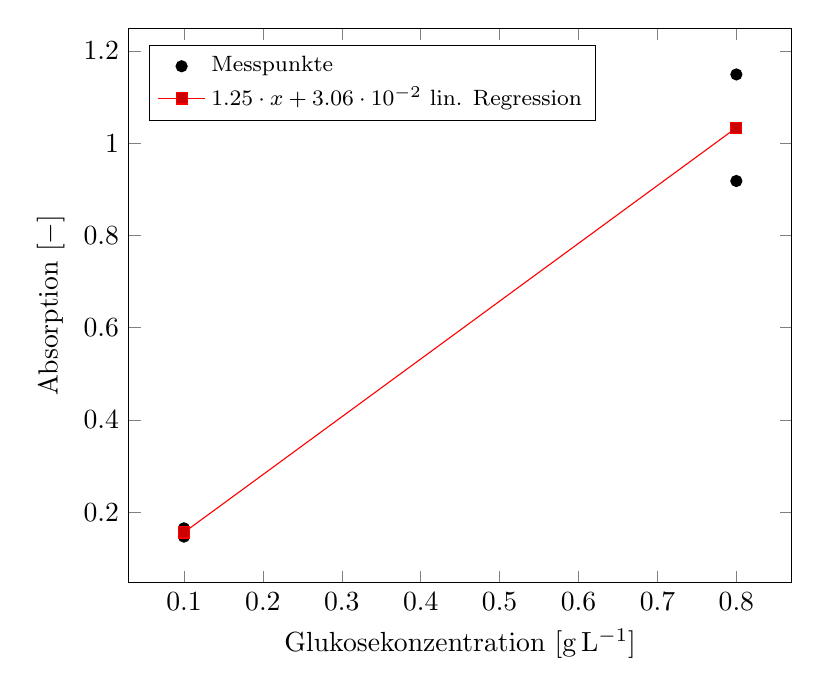
\begin{tikzpicture}
    \pgfplotsset{width=10cm,
        compat=1.3,
        legend style={font=\footnotesize}}
    \begin{axis}[
    xlabel={Glukosekonzentration [\si{\gram\per\liter}]},
    ylabel={Absorption $[-]$},
    legend cell align=left,
    legend pos=north west]
    \addplot[only marks] table[row sep=\\]{
        X Y\\
        0.1 0.147\\
        0.1 0.165\\
        0.8 0.918\\
        0.8 1.149\\
    };
    \addlegendentry{Messpunkte}
    \addplot table[row sep=\\,
    y={create col/linear regression={y=Y}}] % compute a linear regression from the
    %input table
    {
        X Y\\
        0.1 0.147\\
        0.1 0.165\\
        0.8 0.918\\
        0.8 1.149\\
    };
    \addlegendentry{%
        $\pgfmathprintnumber{\pgfplotstableregressiona} \cdot x
        \pgfmathprintnumber[print sign]{\pgfplotstableregressionb}$ lin. Regression} %
    \end{axis}
\end{tikzpicture}



\end{document}
